% Options for packages loaded elsewhere
\PassOptionsToPackage{unicode}{hyperref}
\PassOptionsToPackage{hyphens}{url}
\PassOptionsToPackage{dvipsnames,svgnames,x11names}{xcolor}
%
\documentclass[
  letterpaper,
  DIV=11,
  numbers=noendperiod]{scrreprt}

\usepackage{amsmath,amssymb}
\usepackage{iftex}
\ifPDFTeX
  \usepackage[T1]{fontenc}
  \usepackage[utf8]{inputenc}
  \usepackage{textcomp} % provide euro and other symbols
\else % if luatex or xetex
  \usepackage{unicode-math}
  \defaultfontfeatures{Scale=MatchLowercase}
  \defaultfontfeatures[\rmfamily]{Ligatures=TeX,Scale=1}
\fi
\usepackage{lmodern}
\ifPDFTeX\else  
    % xetex/luatex font selection
\fi
% Use upquote if available, for straight quotes in verbatim environments
\IfFileExists{upquote.sty}{\usepackage{upquote}}{}
\IfFileExists{microtype.sty}{% use microtype if available
  \usepackage[]{microtype}
  \UseMicrotypeSet[protrusion]{basicmath} % disable protrusion for tt fonts
}{}
\makeatletter
\@ifundefined{KOMAClassName}{% if non-KOMA class
  \IfFileExists{parskip.sty}{%
    \usepackage{parskip}
  }{% else
    \setlength{\parindent}{0pt}
    \setlength{\parskip}{6pt plus 2pt minus 1pt}}
}{% if KOMA class
  \KOMAoptions{parskip=half}}
\makeatother
\usepackage{xcolor}
\setlength{\emergencystretch}{3em} % prevent overfull lines
\setcounter{secnumdepth}{5}
% Make \paragraph and \subparagraph free-standing
\makeatletter
\ifx\paragraph\undefined\else
  \let\oldparagraph\paragraph
  \renewcommand{\paragraph}{
    \@ifstar
      \xxxParagraphStar
      \xxxParagraphNoStar
  }
  \newcommand{\xxxParagraphStar}[1]{\oldparagraph*{#1}\mbox{}}
  \newcommand{\xxxParagraphNoStar}[1]{\oldparagraph{#1}\mbox{}}
\fi
\ifx\subparagraph\undefined\else
  \let\oldsubparagraph\subparagraph
  \renewcommand{\subparagraph}{
    \@ifstar
      \xxxSubParagraphStar
      \xxxSubParagraphNoStar
  }
  \newcommand{\xxxSubParagraphStar}[1]{\oldsubparagraph*{#1}\mbox{}}
  \newcommand{\xxxSubParagraphNoStar}[1]{\oldsubparagraph{#1}\mbox{}}
\fi
\makeatother


\providecommand{\tightlist}{%
  \setlength{\itemsep}{0pt}\setlength{\parskip}{0pt}}\usepackage{longtable,booktabs,array}
\usepackage{calc} % for calculating minipage widths
% Correct order of tables after \paragraph or \subparagraph
\usepackage{etoolbox}
\makeatletter
\patchcmd\longtable{\par}{\if@noskipsec\mbox{}\fi\par}{}{}
\makeatother
% Allow footnotes in longtable head/foot
\IfFileExists{footnotehyper.sty}{\usepackage{footnotehyper}}{\usepackage{footnote}}
\makesavenoteenv{longtable}
\usepackage{graphicx}
\makeatletter
\def\maxwidth{\ifdim\Gin@nat@width>\linewidth\linewidth\else\Gin@nat@width\fi}
\def\maxheight{\ifdim\Gin@nat@height>\textheight\textheight\else\Gin@nat@height\fi}
\makeatother
% Scale images if necessary, so that they will not overflow the page
% margins by default, and it is still possible to overwrite the defaults
% using explicit options in \includegraphics[width, height, ...]{}
\setkeys{Gin}{width=\maxwidth,height=\maxheight,keepaspectratio}
% Set default figure placement to htbp
\makeatletter
\def\fps@figure{htbp}
\makeatother
% definitions for citeproc citations
\NewDocumentCommand\citeproctext{}{}
\NewDocumentCommand\citeproc{mm}{%
  \begingroup\def\citeproctext{#2}\cite{#1}\endgroup}
\makeatletter
 % allow citations to break across lines
 \let\@cite@ofmt\@firstofone
 % avoid brackets around text for \cite:
 \def\@biblabel#1{}
 \def\@cite#1#2{{#1\if@tempswa , #2\fi}}
\makeatother
\newlength{\cslhangindent}
\setlength{\cslhangindent}{1.5em}
\newlength{\csllabelwidth}
\setlength{\csllabelwidth}{3em}
\newenvironment{CSLReferences}[2] % #1 hanging-indent, #2 entry-spacing
 {\begin{list}{}{%
  \setlength{\itemindent}{0pt}
  \setlength{\leftmargin}{0pt}
  \setlength{\parsep}{0pt}
  % turn on hanging indent if param 1 is 1
  \ifodd #1
   \setlength{\leftmargin}{\cslhangindent}
   \setlength{\itemindent}{-1\cslhangindent}
  \fi
  % set entry spacing
  \setlength{\itemsep}{#2\baselineskip}}}
 {\end{list}}
\usepackage{calc}
\newcommand{\CSLBlock}[1]{\hfill\break\parbox[t]{\linewidth}{\strut\ignorespaces#1\strut}}
\newcommand{\CSLLeftMargin}[1]{\parbox[t]{\csllabelwidth}{\strut#1\strut}}
\newcommand{\CSLRightInline}[1]{\parbox[t]{\linewidth - \csllabelwidth}{\strut#1\strut}}
\newcommand{\CSLIndent}[1]{\hspace{\cslhangindent}#1}

\KOMAoption{captions}{tableheading}
\makeatletter
\@ifpackageloaded{tcolorbox}{}{\usepackage[skins,breakable]{tcolorbox}}
\@ifpackageloaded{fontawesome5}{}{\usepackage{fontawesome5}}
\definecolor{quarto-callout-color}{HTML}{909090}
\definecolor{quarto-callout-note-color}{HTML}{0758E5}
\definecolor{quarto-callout-important-color}{HTML}{CC1914}
\definecolor{quarto-callout-warning-color}{HTML}{EB9113}
\definecolor{quarto-callout-tip-color}{HTML}{00A047}
\definecolor{quarto-callout-caution-color}{HTML}{FC5300}
\definecolor{quarto-callout-color-frame}{HTML}{acacac}
\definecolor{quarto-callout-note-color-frame}{HTML}{4582ec}
\definecolor{quarto-callout-important-color-frame}{HTML}{d9534f}
\definecolor{quarto-callout-warning-color-frame}{HTML}{f0ad4e}
\definecolor{quarto-callout-tip-color-frame}{HTML}{02b875}
\definecolor{quarto-callout-caution-color-frame}{HTML}{fd7e14}
\makeatother
\makeatletter
\@ifpackageloaded{bookmark}{}{\usepackage{bookmark}}
\makeatother
\makeatletter
\@ifpackageloaded{caption}{}{\usepackage{caption}}
\AtBeginDocument{%
\ifdefined\contentsname
  \renewcommand*\contentsname{Table of contents}
\else
  \newcommand\contentsname{Table of contents}
\fi
\ifdefined\listfigurename
  \renewcommand*\listfigurename{List of Figures}
\else
  \newcommand\listfigurename{List of Figures}
\fi
\ifdefined\listtablename
  \renewcommand*\listtablename{List of Tables}
\else
  \newcommand\listtablename{List of Tables}
\fi
\ifdefined\figurename
  \renewcommand*\figurename{Figure}
\else
  \newcommand\figurename{Figure}
\fi
\ifdefined\tablename
  \renewcommand*\tablename{Table}
\else
  \newcommand\tablename{Table}
\fi
}
\@ifpackageloaded{float}{}{\usepackage{float}}
\floatstyle{ruled}
\@ifundefined{c@chapter}{\newfloat{codelisting}{h}{lop}}{\newfloat{codelisting}{h}{lop}[chapter]}
\floatname{codelisting}{Listing}
\newcommand*\listoflistings{\listof{codelisting}{List of Listings}}
\makeatother
\makeatletter
\makeatother
\makeatletter
\@ifpackageloaded{caption}{}{\usepackage{caption}}
\@ifpackageloaded{subcaption}{}{\usepackage{subcaption}}
\makeatother

\ifLuaTeX
  \usepackage{selnolig}  % disable illegal ligatures
\fi
\usepackage{bookmark}

\IfFileExists{xurl.sty}{\usepackage{xurl}}{} % add URL line breaks if available
\urlstyle{same} % disable monospaced font for URLs
\hypersetup{
  pdftitle={Cognitive Neuroscience 2425},
  pdfauthor={Javier Ortiz-Tudela},
  colorlinks=true,
  linkcolor={blue},
  filecolor={Maroon},
  citecolor={Blue},
  urlcolor={Blue},
  pdfcreator={LaTeX via pandoc}}


\title{Cognitive Neuroscience 2425}
\author{Javier Ortiz-Tudela}
\date{2025-01-01}

\begin{document}
\maketitle

\renewcommand*\contentsname{Table of contents}
{
\hypersetup{linkcolor=}
\setcounter{tocdepth}{2}
\tableofcontents
}

\bookmarksetup{startatroot}

\chapter{Welcome to Cognitive
Neuroscience}\label{welcome-to-cognitive-neuroscience}

This book contains the materials for the small group session of the
Cognitive Neuroscience course (Academic year 2425). The overarching aim
of these sessions is to gain in-depth knowledge about certain sub-topics
in Cognitive Neuroscience which, due to time limitation, cannot be
covered in detail in the big group sessions. The final outcome will be a
group project in which you will create a podcast-like episode on a
subtopic of your chosing within Cognitive Neuroscience.

\begin{figure}[H]

{\centering 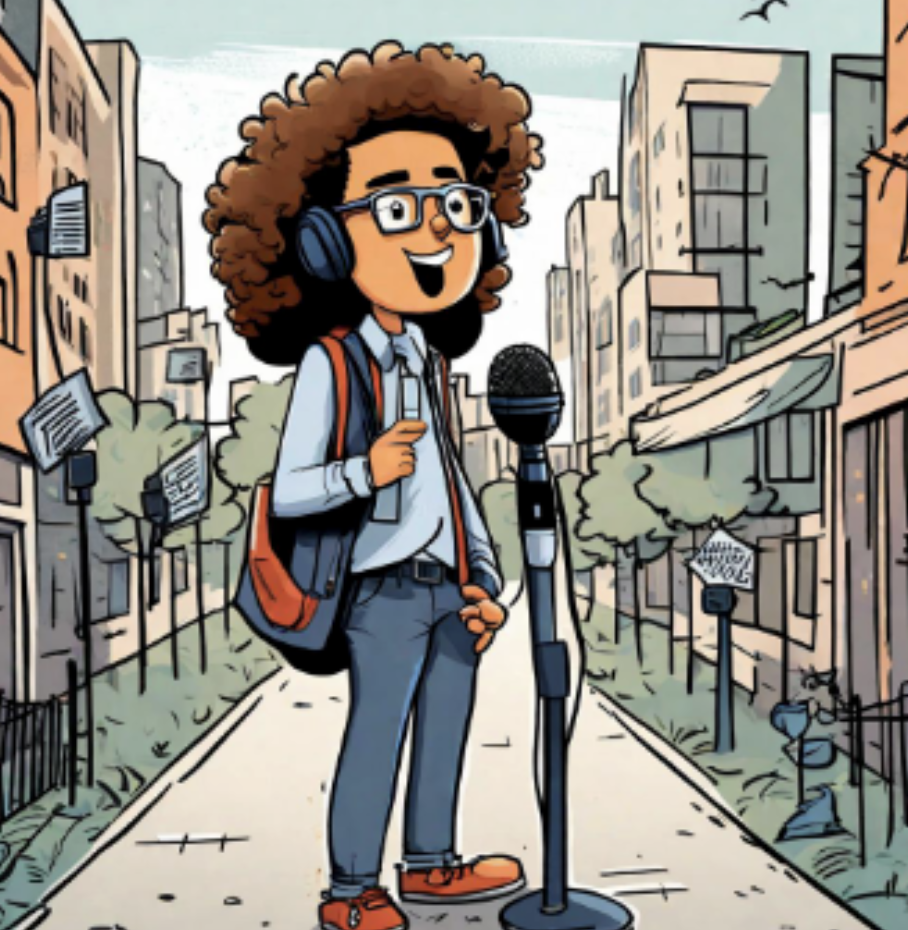
\includegraphics{_images/podcaster.png}

}

\caption{The image of a happy and dynamic podcaster recording in a very
bad scenario. Be motivated by this guy, but do not be this guy.
Recording outdoors is a very bad idea.}

\end{figure}%

\section{How to Use This Book}\label{how-to-use-this-book}

This book is organized week by week, following the course structure.
Each chapter contains information about what is to be expected for the
corresponding week's session. Also, throughout the weeks you will find
information about concrete milestones and how to deliver them.

Navigate through the chapters using the sidebar or the next/previous
buttons at the bottom of each page.

If you have any questions or need further clarification on the course
content, assignments, or any technical issues related to podcast
production, please do not hesitate to reach out to the course
instructors via email or during office hours. We are here to support
your learning journey and ensure you have all the resources you need to
succeed in this course.

Remember, this course is not just about learning theoretical aspects of
Cognitive Neuroscience but also about learning to communicate this
knowledge in a creative and practical way. We encourage you to engage
actively with the course materials, participate in discussions during
the on-site sessions, and bring your unique perspectives to the episodes
you will create.

Good luck, and we look forward to hearing your podcasts!

\part{Course Information}

\chapter{Introduction to Cognitive Neuroscience and the Podcast
Project}\label{introduction-to-cognitive-neuroscience-and-the-podcast-project}

Welcome to the small group sessions of the Cognitive Neuroscience
course! These sessions are conceived to be a learning experience which
combines in-depth study of some key areas of cognitive neuroscience with
the practical application of science communication through podcast
creation.

\section{Course Overview}\label{course-overview}

This course is designed as a 13-week journey that will take you through
all the necessary steps starting from coming out with a scientific
question, finding information about it, critically thinking about this
information, and to eventually create a summary of the learned
information in audio format. Throughout the semester, you will work in
groups of 3-4 students to create a 5-10 minute podcast episode on a
specific subtopic within cognitive neuroscience.

\section{Course Objectives}\label{course-objectives}

By the end of this course, you will:

\begin{enumerate}
\def\labelenumi{\arabic{enumi}.}
\tightlist
\item
  Gain in-depth knowledge in a specific area within Cognitive
  Neuroscience
\item
  Learn to review, critically analyze and synthesize scientific
  literature
\item
  Gain experience in interviewing experts scientists in the field
\item
  Develop proficiency in sythesizing and communicating scientific
  information to diverse audiences
\item
  Acquire basic skills in recording and editing audio content generally
  and on podcast production more concretely
\item
  Enhance your teamwork and project management skills
\end{enumerate}

\section{Course Instructors}\label{course-instructors}

\begin{itemize}
\tightlist
\item
  \textbf{Javier Ortiz Tudela}

  \begin{itemize}
  \tightlist
  \item
    Email: ortiztudela@ugr.es
  \item
    Office: 308 at CIMCYC
  \end{itemize}
\item
  \textbf{María Ruz}

  \begin{itemize}
  \tightlist
  \item
    Email: mruz@ugr.es
  \item
    Office: 4 at CIMCYC
  \end{itemize}
\end{itemize}

Note: While we have office hours, it's usually better if you send us an
email in advance so that we can prepare for your questions.

\section{Getting Started}\label{getting-started}

As we embark on this journey together, keep an open mind, be curious,
and \emph{don't be afraid to ask questions}. Cognitive neuroscience is
fascinating and complex, and your task is to make it accessible and
engaging for the audience.

In the next section, we'll dive into the course roadmap, giving you a
clear picture of what to expect in the coming weeks.

\part{Weekly Content}

\chapter{Week 0: Course Kick-off}\label{week-0-course-kick-off}

\section{Course Structure}\label{course-structure}

The course is structured week-by-week, guiding you through the process
of creating your podcast. Each week focuses on specific tasks and
milestones, building towards your final product. The workload is
distributed between in-person sessions and autonomous group work.

During the in-person sessions we will explain each step in the process
and present you with strategies and tools so that you can work
efficiently. In addition, some of the in-person time will be dedicated
for group work so that you can complement your autonomous work. If you
regularly attend the in-person sessions and you deliver all the
milestones in their due time, the amount of autonomous work should be
minimal.

\subsection{Let's start at the end (product): Your own CogNeuro
Podcast!}\label{lets-start-at-the-end-product-your-own-cogneuro-podcast}

The main project of this course is to create a 5 to 10-minute
podcast-like recording on a subtopic within Cognitive Neuroscience.
Throughout the semester, you'll work through various milestones, from
topic selection to the final production of your podcast episode. If you
have never worked on a similar project, rest assure, we will walk you
through all the steps so that, if you follow along, you will be able to
complete the assignment in time.

We will give you a set of broad topics for you to choose from but you
will also be able (and encouraged!) to work on a different topic that
you find more interesting. If you want to have a more concrete idea of
what we are expecting from you, here you can find some of the episodes
that were created in the 2324 edition (shared with permission form the
authors).

\begin{itemize}
\tightlist
\item
  \href{_examples/Tue_11-12_Poverty.mp3}{Poverty}
\item
  \href{_examples/Tue_11-12_Neurosexism.mp3}{Neurosexism}
\item
  \href{_examples/Wed_12-13_Stereotypes-1.mp3}{Stereotypes}
\item
  \href{_examples/Wed_18-19_Consciencia-1.mp3}{Consciencia}
\item
  \href{_examples/Wed_18-19_Neurosexismo.mp3}{Neurosexismo}
\item
  \href{_examples/Wed_18-19_Plasticidad-1.mp3}{Plasticidad}
\end{itemize}

\subsection{How We'll Achieve This}\label{how-well-achieve-this}

\begin{itemize}
\tightlist
\item
  Work in small groups arranged according to topic preferences.
\item
  Follow a weekly program covering all necessary steps.
\item
  Engage in lots of in-session work.
\item
  Complete partial milestones throughout the semester.
\item
  Participate in joint listening sessions of the recordings, Q\&A, and
  feedback.
\end{itemize}

Here you will find a detailed plan of what we will do on each session
(this file will also be available on PRADO).

\begin{tcolorbox}[enhanced jigsaw, toptitle=1mm, colbacktitle=quarto-callout-note-color!10!white, breakable, leftrule=.75mm, titlerule=0mm, colframe=quarto-callout-note-color-frame, opacityback=0, arc=.35mm, opacitybacktitle=0.6, colback=white, title=\textcolor{quarto-callout-note-color}{\faInfo}\hspace{0.5em}{Roadmap for the Course}, toprule=.15mm, bottomtitle=1mm, coltitle=black, rightrule=.15mm, bottomrule=.15mm, left=2mm]

\subsubsection{Week 0: Course Introduction and
Roadmap}\label{week-0-course-introduction-and-roadmap}

\begin{itemize}
\tightlist
\item
  \textbf{Date:} September 18th
\item
  \textbf{Activities:} In this introductory session, we'll go over the
  course objectives and what you can expect to achieve by the end. We
  will also cover our expected timeline, deliverable milestones and how
  we will evaluate your work.
\end{itemize}

\subsubsection{Week 1: Topic Selection and
Research}\label{week-1-topic-selection-and-research}

\begin{itemize}
\tightlist
\item
  \textbf{Date:} September 25th
\item
  \textbf{Activities:}

  \begin{itemize}
  \tightlist
  \item
    Presentation of the skeptical watchlist for Cognitive Neuroscience
    research.
  \item
    Introduction to available topics along with the selected papers.
  \item
    Students rate their topic preferences
    (https://forms.gle/vv24vQnko35txwyt8)
  \item
    Formation of groups based on topic preferences.
  \end{itemize}
\end{itemize}

\subsubsection{Week 2: In-depth Research (Part
1)}\label{week-2-in-depth-research-part-1}

\begin{itemize}
\tightlist
\item
  \textbf{Date:} September 25th
\item
  \textbf{Activities:}

  \begin{itemize}
  \tightlist
  \item
    Read and analyze the proposed paper for the selected topic.
  \item
    Conduct topic-specific literature searches.
  \item
    Distribute additional papers among group members and start reading.
  \end{itemize}
\end{itemize}

\subsubsection{Week 3: In-depth Research (Part
2)}\label{week-3-in-depth-research-part-2}

\begin{itemize}
\tightlist
\item
  \textbf{Date:} October 2nd
\item
  \textbf{Activities:}

  \begin{itemize}
  \tightlist
  \item
    Continue reading and analyzing the literature.
  \item
    Present findings to peers and discuss.
  \item
    Identify interesting subtopics for further exploration.
  \item
    Present popular science podcasts as examples.
  \item
    \textbf{Milestone:} Decide on a subtopic, a target audience and
    provide a tentative title for your podcast episode.
  \end{itemize}
\end{itemize}

\subsubsection{Week 4: Episode Outline}\label{week-4-episode-outline}

\begin{itemize}
\tightlist
\item
  \textbf{Date:} October 9th
\item
  \textbf{Activities:}

  \begin{itemize}
  \tightlist
  \item
    Continue refining the content through additional reading.
  \item
    Develop an outline for the podcast episode collaboratively.
  \item
    Decide on the tone (formal, light, fun) of the episode.
  \item
    Assign roles for the final episode (who will speak, etc.).
  \item
    Begin working individually on respective sections.
  \item
    Seek guidance and feedback as needed.
  \end{itemize}
\end{itemize}

\subsubsection{Week 5: Preparing
Interviews}\label{week-5-preparing-interviews}

\begin{itemize}
\tightlist
\item
  \textbf{Date:} October 16th
\item
  \textbf{Activities:}

  \begin{itemize}
  \tightlist
  \item
    Identify and research the expert for the interview.
  \item
    Decide on the format for the interview (audio recording or
    discussion).
  \item
    Develop and select key questions for the interview.
  \item
    Integrate the interview into the episode outline.
  \item
    \textbf{Milestone:} Send the outline and questions for review.
  \end{itemize}
\end{itemize}

\subsubsection{Week 6: Recording Interviews (Part 1) + Script Writing
(Part
1)}\label{week-6-recording-interviews-part-1-script-writing-part-1}

\begin{itemize}
\tightlist
\item
  \textbf{Date:} October 23rd
\item
  \textbf{Activities:}

  \begin{itemize}
  \tightlist
  \item
    Begin recording interviews with the experts.
  \item
    Learn tips for writing engaging introductions and conclusions.
  \item
    Start writing the script for the episode.
  \item
    Seek guidance and feedback as needed.
  \end{itemize}
\end{itemize}

\subsubsection{Week 7: Recording Interviews (Part 2) + Script Writing
(Part
2)}\label{week-7-recording-interviews-part-2-script-writing-part-2}

\begin{itemize}
\tightlist
\item
  \textbf{Date:} October 30th
\item
  \textbf{Activities:}

  \begin{itemize}
  \tightlist
  \item
    Continue recording interviews.
  \item
    Review and adjust the episode outline if necessary.
  \item
    Continue writing the script.
  \item
    \textbf{Milestone:} Send script draft for review.
  \end{itemize}
\end{itemize}

\subsubsection{Week 8: Script Writing (Part 3) + Intro to
Recording}\label{week-8-script-writing-part-3-intro-to-recording}

\begin{itemize}
\tightlist
\item
  \textbf{Date:} November 6th
\item
  \textbf{Activities:}

  \begin{itemize}
  \tightlist
  \item
    Introduction to podcast recording techniques.
  \item
    Discussion on the importance of recording environment and speaker
    articulation and delivery.
  \item
    Basic audio recording tools.
  \item
    Incorporate insights from interviews into the episode.
  \item
    Continue refining the script based on feedback.
  \end{itemize}
\end{itemize}

\subsubsection{Week 9: Script Writing (Part 4) + Intro to
Editing}\label{week-9-script-writing-part-4-intro-to-editing}

\begin{itemize}
\tightlist
\item
  \textbf{Date:} November 13th
\item
  \textbf{Activities:}

  \begin{itemize}
  \tightlist
  \item
    Introduction to podcast editing techniques.
  \item
    Discussion on the use of transitions, sound effects, and music.
  \item
    Basic audio editing tools.
  \item
    Incorporate insights from interviews into the episode.
  \item
    Continue refining the script based on feedback.
  \end{itemize}
\end{itemize}

\subsubsection{Week 10: Recording and Audio Editing (Part
1)}\label{week-10-recording-and-audio-editing-part-1}

\begin{itemize}
\tightlist
\item
  \textbf{Date:} November 20th
\item
  \textbf{Activities:}

  \begin{itemize}
  \tightlist
  \item
    Start recording the episode using the developed script.
  \item
    Seek guidance and feedback as needed.
  \end{itemize}
\end{itemize}

\subsubsection{Week 11: Recording and Audio Editing (Part
2)}\label{week-11-recording-and-audio-editing-part-2}

\begin{itemize}
\tightlist
\item
  \textbf{Date:} November 27th
\item
  \textbf{Activities:}

  \begin{itemize}
  \tightlist
  \item
    Continue recording.
  \item
    Support in editing the recorded audio for clarity and coherence.
  \item
    Review and revise the entire podcast episode as a group.
  \item
    Make necessary edits to enhance the episode's flow and quality.
  \end{itemize}
\end{itemize}

\subsubsection{Week 12: Podcast Presentation and Group Feedback (Part
I)}\label{week-12-podcast-presentation-and-group-feedback-part-i}

\begin{itemize}
\tightlist
\item
  \textbf{Date:} November 4th
\item
  \textbf{Activities:}

  \begin{itemize}
  \tightlist
  \item
    Listen to the final version of the episodes as a group.
  \item
    Q\&A session with other groups.
  \item
    Provide and receive constructive feedback on various aspects of the
    episode.
  \item
    Vote on different aspects of the podcast (e.g., content, clarity)
  \item
    Discuss feedback and the overall experience.
  \end{itemize}
\end{itemize}

\end{tcolorbox}

\section{Resources}\label{resources}

\subsection{Technical Resources}\label{technical-resources}

\begin{itemize}
\tightlist
\item
  This book!
\item
  PRADO platform
\item
  Audio recording software
\item
  Audio editing software
\item
  A regular personal-use computer
\end{itemize}

\subsection{Human Resources (for
interviews)}\label{human-resources-for-interviews}

\begin{itemize}
\tightlist
\item
  Your peers!
\item
  Researchers from the UGR (PhD students, Postdoctoral researchers, Full
  Professors)
\end{itemize}

\section{Evaluation}\label{evaluation}

Your total grade in this project (which will be 30\% of the final grade
of the semester) will be divided into two components:

\begin{enumerate}
\def\labelenumi{\arabic{enumi}.}
\tightlist
\item
  \textbf{Milestones (3 points)} Three deliverables for intermediate
  steps:

  \begin{itemize}
  \tightlist
  \item
    Topic selection and title (Week 3) - 1 point
  \item
    Episode outline (Week 5) - 1 point
  \item
    Script draft (Week 7) - 1 point
  \end{itemize}
\end{enumerate}

We will set specific deadlines for each one of them. In order to get the
full mark for each of the milestones, you must submit your assignment
before the deadline. We will apply a penalti of 50\% for submissions
delays \textless{} 24h and of 100\% for submission delays \textgreater{}
24h.

\begin{enumerate}
\def\labelenumi{\arabic{enumi}.}
\setcounter{enumi}{1}
\tightlist
\item
  \textbf{Final Episode (7 points)} Key aspects considered:

  \begin{itemize}
  \tightlist
  \item
    Clarity and coherence of the content
  \item
    Correct interpretation and integration of the data and ideas
  \item
    Format and engagement
  \item
    Recording and editing quality
  \end{itemize}
\end{enumerate}

\subsection{Podcast Evaluation
Criteria}\label{podcast-evaluation-criteria}

\begin{longtable}[]{@{}
  >{\raggedright\arraybackslash}p{(\columnwidth - 10\tabcolsep) * \real{0.1071}}
  >{\raggedright\arraybackslash}p{(\columnwidth - 10\tabcolsep) * \real{0.2381}}
  >{\raggedright\arraybackslash}p{(\columnwidth - 10\tabcolsep) * \real{0.1786}}
  >{\raggedright\arraybackslash}p{(\columnwidth - 10\tabcolsep) * \real{0.1786}}
  >{\raggedright\arraybackslash}p{(\columnwidth - 10\tabcolsep) * \real{0.1190}}
  >{\raggedright\arraybackslash}p{(\columnwidth - 10\tabcolsep) * \real{0.1786}}@{}}
\toprule\noalign{}
\begin{minipage}[b]{\linewidth}\raggedright
Criteria
\end{minipage} & \begin{minipage}[b]{\linewidth}\raggedright
1 (Unacceptable)
\end{minipage} & \begin{minipage}[b]{\linewidth}\raggedright
2 (Deficient)
\end{minipage} & \begin{minipage}[b]{\linewidth}\raggedright
3 (Acceptable)
\end{minipage} & \begin{minipage}[b]{\linewidth}\raggedright
4 (Good)
\end{minipage} & \begin{minipage}[b]{\linewidth}\raggedright
5 (Excellent)
\end{minipage} \\
\midrule\noalign{}
\endhead
\bottomrule\noalign{}
\endlastfoot
\textbf{Clarity and Coherence} \emph{(2 points)} & The content is
confusing and difficult to follow; lacks a clear focus. & The content
has some moments of clarity, but overall is difficult to understand. &
There is a logical sequence for the most part with some moments of
ambiguity. & The content is clear and well articulated throughout most
of the podcast. & The content is extremely clear and easy to follow
throughout the entire podcast. \\
\textbf{Data Interpretation} \emph{(2 points)} & Total lack of or
erroneous interpretation of data. & Basic interpretation of data, but
with significant errors or misunderstandings. & Correct interpretation
of data, but lacks depth or analysis. & Good interpretation of data with
detailed analysis. & Exceptional interpretation and profound analysis of
the presented data. \\
\textbf{Dynamics} \emph{(2 points)} & The content is too dense and/or
the format is not suitable for the content. & The format is correct but
lacks attentional cues for the audience. & The format is adequate and
includes some attentional cues. & The format is adequate and the
attentional cues maintain the listener's attention. & The format is
ideal and novel; attentional cues make the content integrate fluidly. \\
\textbf{Production} \emph{(1 point)} & Poor audio quality and careless
editing; constant technical distractions. & Fair audio quality and
editing, but with several distractions. & Adequate audio quality and
editing, with few distractions. & High-quality audio and professional
editing; minimal distractions. & Exceptional audio quality and editing;
professional-grade production with no distractions. \\
\end{longtable}

Additionally, we will be awarding prizes in categories such as
\emph{``Most Interesting Episode''}, \emph{``Most Fun Episode''}, and
\emph{``Best Recorded Episode''} based on the votes of your peers. Each
prize will add a 0.2 bonus to your whichever mark your podcast got
according to the evaluation criteria (up to a maximum of 7 points).

\section{Topics}\label{topics}

We have selected one research paper as a starting point for each topic.
You will find these papers below and also on PRADO. The main topics
include:

\begin{itemize}
\tightlist
\item
  \textbf{Neuroanatomy and plasticity}: (Merabet and Pascual-Leone 2010)
\item
  \textbf{Consciousness}: (Sohn 2019)
\item
  \textbf{Brain stimulation}: (Yavari et al. 2018)
\item
  \textbf{Poverty}: (Farah 2017)
\item
  \textbf{Neurosexism}: (Meynell 2013)
\item
  \textbf{Stereotypes and prejudices}: (Amodio 2014)
\end{itemize}

\section{Next Steps}\label{next-steps}

In the coming weeks, you will dive deeper into one of these topics. You
will learn about the parts that you find more interesting and attempt at
integrating them together with your work group. The ultimate goal is
that you can efficiently communicate all that information to the rest of
your classmates. As a bonus, you will also get to learn from their work
on the things that they find fascinating! Be prepared to engage in
collaborative work, conduct in-depth research, develop your science
communication skills, and learn to provide (and to receive) constructive
feedback.

\subsection{References}\label{references}

\chapter{Week 1: Topic Selection and
Research}\label{week-1-topic-selection-and-research-1}

\section{Objectives}\label{objectives}

By the end of this week, students will:

\begin{itemize}
\tightlist
\item
  Have a quick recap of the goal of the course to get new students on
  board
\item
  Be introduced to potential pitfalls in Cognitive Neuroscience research
\item
  Select their preferred topics
\item
  Be assigned to groups based on their preferences
\end{itemize}

\section{Milestones and Delivery
Dates}\label{milestones-and-delivery-dates}

We'll review the project milestones and their expected delivery dates.
This will help you plan your work and ensure you stay on track
throughout the course.

\section{A Skeptical Approach to Cognitive Neuroscience
Research}\label{a-skeptical-approach-to-cognitive-neuroscience-research}

In this section, we'll discuss common pitfalls and areas of caution in
Cognitive Neuroscience research. This ``skeptical watchlist'' will help
you approach your research with a critical eye and ensure the scientific
integrity of your podcast content.

You can find the slides for this section below.

\section{Tasks}\label{tasks}

\begin{enumerate}
\def\labelenumi{\arabic{enumi}.}
\tightlist
\item
  Review the available topics and associated papers.
\item
  Consider your interests and rate your preferences for the different
  topics.
\end{enumerate}

\section{Next Steps}\label{next-steps-1}

In the coming weeks, you'll dive deeper into your chosen topic, conduct
in-depth research, and begin planning your podcast episode. Start
thinking about what aspects of your topic you find most intriguing and
what questions you'd like to explore further.

\chapter{Week 2: In-depth Research (Part
1)}\label{week-2-in-depth-research-part-1-1}

\section{Objectives}\label{objectives-1}

By the end of this week, you will:

\begin{itemize}
\tightlist
\item
  Establish initial communication within their respective grops
\item
  Understand how to conduct topic-specific literature searches
\item
  Distribute tasks among group members (reading, recording, editing,
  speaking, interviewing)
\item
  Begin in-depth reading on their chosen topic
\end{itemize}

\subsection{Key Ideas from Previous
Weeks}\label{key-ideas-from-previous-weeks}

\begin{itemize}
\tightlist
\item
  The recording should \textbf{not} be a formal presentation of a paper
\item
  Use the skeptical watchlist while researching (available on this book
  and on PRADO)
\end{itemize}

\section{Group Formation}\label{group-formation}

\begin{itemize}
\tightlist
\item
  Groups have been created based on your 1st or 2nd choice preferences
\item
  Each group consists of 3-5 members for balanced workload and
  efficiency
\item
  Reach out to your group members and start collaborating
\item
  Be mindful of others' needs and ensure everyone feels comfortable
\item
  If you encounter any issues, please reach out to us for solutions
\end{itemize}

\section{In-depth Research}\label{in-depth-research}

\subsection{Getting Started}\label{getting-started-1}

We gave you an initial paper for each one of the topics. Now it is time
to review the one for your topic so that you can pull out some ideas and
some more refereces that can guide you deeper into a concrete direction.
Here are a few questions that might help you extract the relevant
information from the paper:

\begin{itemize}
\tightlist
\item
  What's the main focus of the article?
\item
  Which sections interest you most?
\item
  Do you need additional context to understand certain parts?
\item
  What other studies inspired the authors?
\end{itemize}

\subsection{Finding Additional
Resources}\label{finding-additional-resources}

When conducting online scientific literature searches, you have several
options, each with its own trade-offs between search time and output
validation time.

\begin{enumerate}
\def\labelenumi{\arabic{enumi}.}
\tightlist
\item
  Traditional Databases

  \begin{itemize}
  \tightlist
  \item
    Platforms like Scopus and PubMed offer comprehensive, curated
    collections of scientific literature.
  \item
    These databases typically require more search time but provide
    highly reliable, peer-reviewed results.
  \end{itemize}
\item
  Google Scholar

  \begin{itemize}
  \tightlist
  \item
    A popular middle-ground option that balances search speed and result
    breadth.
  \item
    It offers a user-friendly interface and wide coverage across various
    disciplines.
  \item
    While faster than traditional databases, it may include some
    non-peer-reviewed content.
  \end{itemize}
\item
  AI-Powered Tools

  \begin{itemize}
  \tightlist
  \item
    Emerging platforms like Consensus use artificial intelligence to
    streamline the search process.
  \item
    These tools significantly reduce search time but may require
    additional effort to validate outputs.
  \end{itemize}
\end{enumerate}

Validation of search results is crucial, especially when using faster,
more inclusive search methods. Google Scholar may include
non-peer-reviewed materials, preprints, or even non-academic sources,
which can affect the reliability of your research if not properly
vetted. AI-powered tools, while efficient, may occasionally
``hallucinate'' or generate inaccurate information, particularly when
dealing with specific data points or less common topics. These tools
might also misinterpret context or nuance in complex scientific
discussions. Therefore, it's essential to cross-reference findings,
verify sources, and critically evaluate the relevance and accuracy of
search results, regardless of the platform used.

\begin{figure}[H]

{\centering 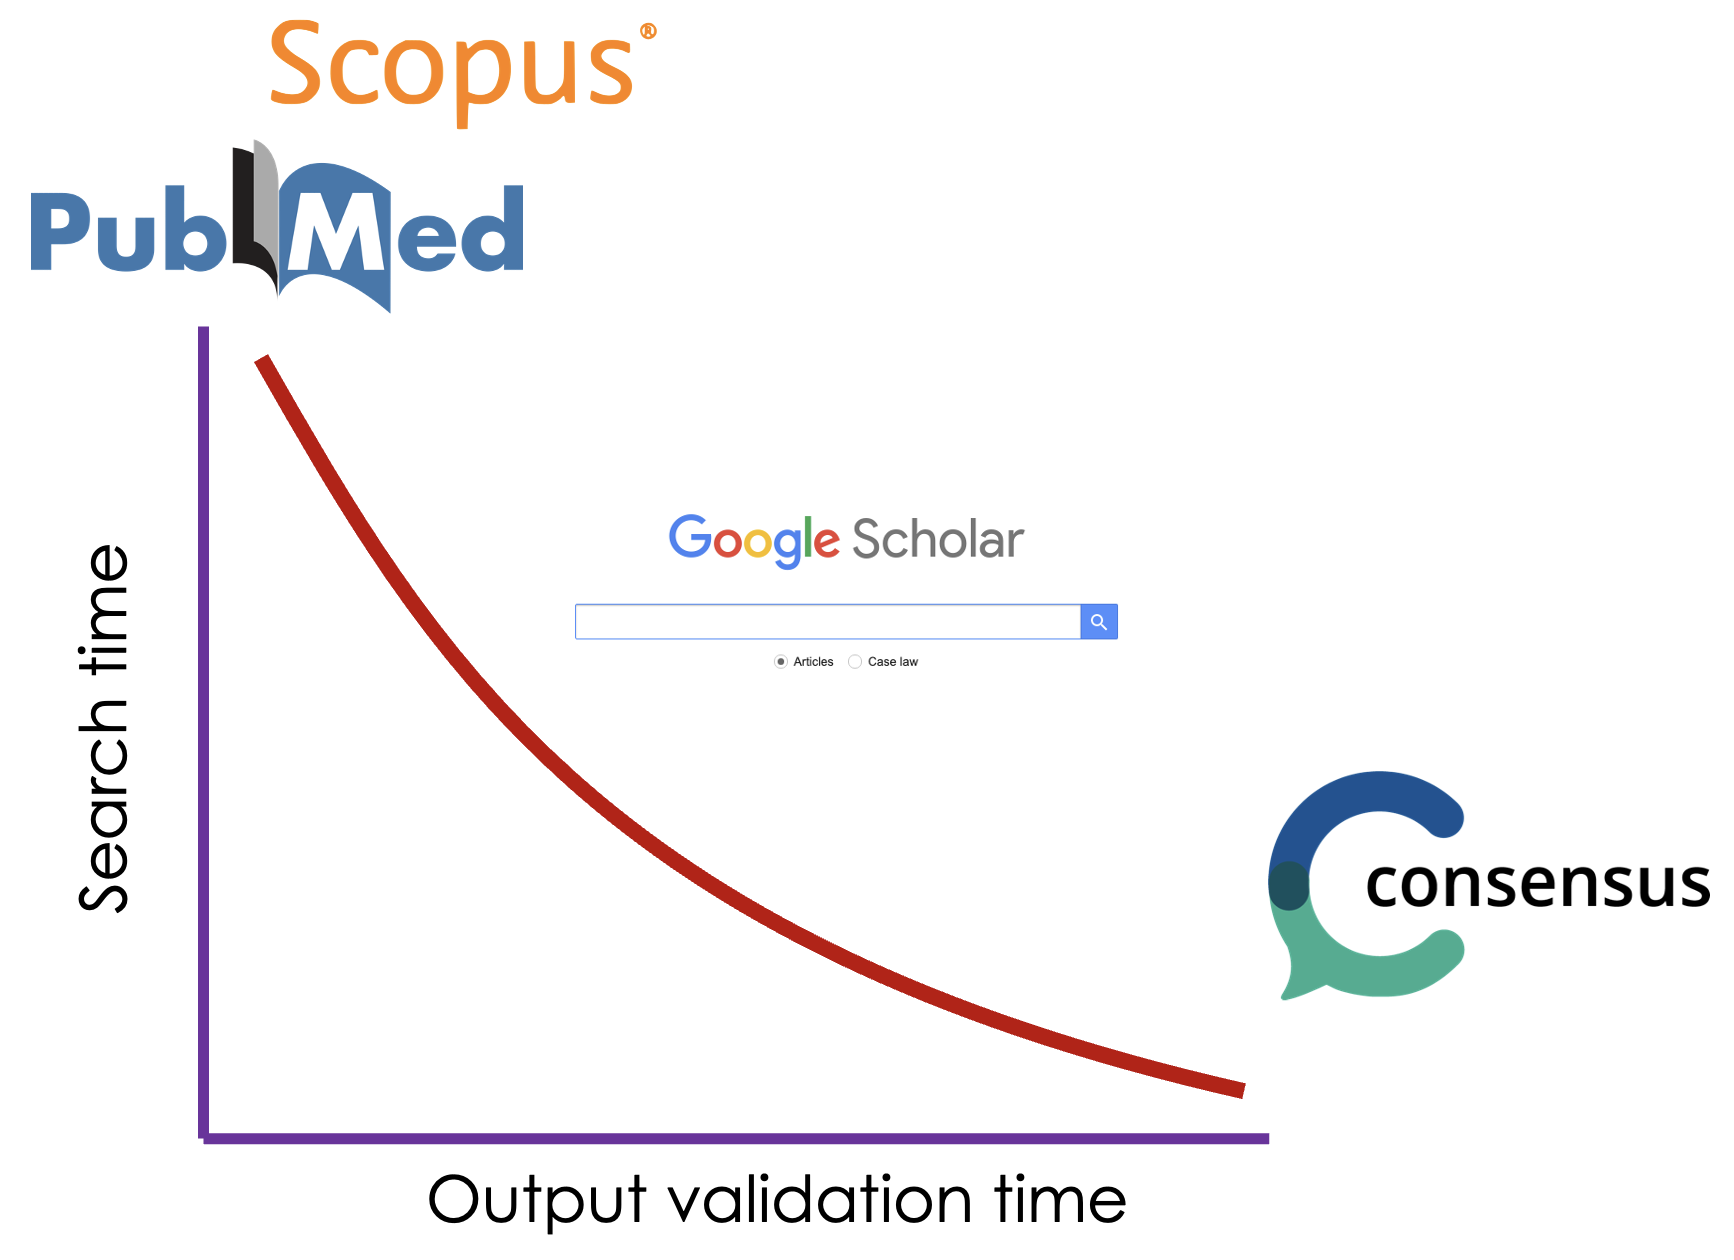
\includegraphics{_images/search_engines.png}

}

\caption{Schematic depiction of the trade off between search time and
validation time}

\end{figure}%

When choosing a search method, consider your research needs:

\begin{itemize}
\tightlist
\item
  For thorough, highly validated results, traditional databases may be
  preferable.
\item
  For quick, broad searches, Google Scholar offers a good balance.
\item
  For rapid literature reviews or initial explorations, AI-powered tools
  can be valuable, but exercise caution and verify findings.
\end{itemize}

Remember, the faster the search process, the more time you might need to
spend validating the results. Choose the approach that best fits your
research goals and time constraints, and always maintain a critical eye
when reviewing your findings.

\subsection{Accessing papers:}\label{accessing-papers}

\begin{itemize}
\tightlist
\item
  Use university network or VPN for paywalled journals
\item
  Try different versions if available
\item
  Reach out to us if you can't access a paper
\end{itemize}

\subsection{Alternative Research
Methods}\label{alternative-research-methods}

Explore other platforms for ideas as well as for information:

\begin{itemize}
\item
  YouTube channels (e.g.,
  \href{https://www.youtube.com/@kurzgesagt}{kurzgesagt},
  \href{https://www.youtube.com/@AsapSCIENCE}{AsapSCIENCE},
  \href{https://www.youtube.com/@WIRED}{WIRED})
\item
  Podcasts (e.g., \href{https://braininspired.co/}{Brain Inspired},
  \href{https://startalkmedia.com/}{StarTalk},
  \href{https://lexfridman.com/podcast/}{Lex Fridman Podcast})
\end{itemize}

Remember to use your skeptical watchlist when exploring these sources!

\section{Tasks for This Week}\label{tasks-for-this-week}

\begin{enumerate}
\def\labelenumi{\arabic{enumi}.}
\tightlist
\item
  Connect with your group members
\item
  Review the suggested paper for your topic
\item
  Conduct initial literature searches
\item
  Distribute reading tasks among group members
\item
  Begin in-depth reading of your assigned materials
\end{enumerate}

\section{Potential questions we
anticipate}\label{potential-questions-we-anticipate}

\textbf{Q: How many papers do we need to read?}\\
A: There's no set minimum or maximum. Focus on quality and relevance.

\textbf{Q: What if I find conflicting information in different
papers?}\\
A: This is normal in science! Use your skeptical watchlist to evaluate
the papers' credibility. If you can't decide, consider discussing both
perspectives in your podcast -- competing accounts are part of
scientific progress.

\section{Next Steps}\label{next-steps-2}

In the next week, we'll focus on narrowing down your topic into a
central and manageable idea and on defining your target audience.

\chapter{Week 3: In-depth Research (Part
2)}\label{week-3-in-depth-research-part-2-1}

\section{Objectives}\label{objectives-2}

By the end of this week, you will have to submit \textbf{the first
milestone}. This will be the one of the most important steps in your
podcast creation: you have to decide on the topic of the podcast, frame
it for a concrete target audience and provide a tentative title.

\subsection{Key Ideas from Previous
Weeks}\label{key-ideas-from-previous-weeks-1}

\begin{itemize}
\tightlist
\item
  Decide on a sub-topic within your main topic
\item
  Attribute different roles to group members is a great way to maximize
  efficiency
\item
  The recording should \textbf{not} be a formal presentation of a paper
\item
  Use the skeptical watchlist while researching (available on this book
  and on PRADO)
\end{itemize}

\section{In-depth Research II}\label{in-depth-research-ii}

By now, you should already have, at least, a tentative idea of what you
want to talk about. Now, it is time to further fine-tune that idea to
make it more concrete. Keep in mind that the final product will have a
maximum duration of 10 minutes. Thus you should strive for either:

\begin{itemize}
\tightlist
\item
  Cover a narrow sub-topic within the broader umbrella topic you were
  assigned to
\item
  Provide a shallower overview of a broad topic.
\end{itemize}

Both options are totally fine as long as you find it interesting (and
that you are able to communicate your enthusiasm to the audience). Keep
these two options in mind while digging through research so you can
decide where to focus your effors.

\section{Defining Your Podcast
Audience}\label{defining-your-podcast-audience}

When creating a science-based podcast (or any kind of podcast, tbh), one
of the most crucial decisions you'll make is choosing your target
audience. This choice should be made early in the planning process, as
it will significantly influence various aspects of your podcast,
including content, format, tone, and language.

\subsection{Why Audience Matters}\label{why-audience-matters}

\begin{enumerate}
\def\labelenumi{\arabic{enumi}.}
\item
  Content Depth: The level of detail and complexity in your discussions
  will vary greatly depending on whether you're addressing neuroscience
  specialists or the general public.
\item
  Language Use: Technical jargon appropriate for scientists might
  confuse a lay audience, while oversimplification could bore experts.
\item
  Topic Selection: Your audience's background knowledge and interests
  will guide which topics are most relevant and engaging.
\item
  Format and Style: The podcast's structure, length of the sections, and
  presentation style should cater to your audience's preferences and
  listening habits.
\end{enumerate}

\subsection{Potential Target
Audiences}\label{potential-target-audiences}

Consider these example audience categories to aid your definition of
your podcast's focus:

\begin{enumerate}
\def\labelenumi{\arabic{enumi}.}
\tightlist
\item
  Specialist Neuroscientists:

  \begin{itemize}
  \tightlist
  \item
    Highly technical content
  \item
    In-depth discussions of current research
  \item
    Use of field-specific terminology
  \end{itemize}
\item
  General Scientists:

  \begin{itemize}
  \tightlist
  \item
    Broader scientific context
  \item
    Interdisciplinary connections
  \item
    Less neuroscience-specific jargon
  \end{itemize}
\item
  Psychologists without Scientific Background:

  \begin{itemize}
  \tightlist
  \item
    Focus on practical applications
  \item
    Simplified explanations of neuroscientific concepts
  \item
    Connections to psychological theories and practices
  \end{itemize}
\item
  General Population:

  \begin{itemize}
  \tightlist
  \item
    Emphasis on relatable examples and real-world implications
  \item
    Clear, jargon-free explanations
  \item
    More time spent on foundational concepts
  \end{itemize}
\end{enumerate}

This list is not exhaustive and other types of audiences can be
considered. But bear in mind that by clearly defining your target
audience in advance, you can create a more focused, engaging, and
effective product. This clarity will guide your content creation process
and help you build an engaging episode.

\section{Tasks for This Week}\label{tasks-for-this-week-1}

\begin{enumerate}
\def\labelenumi{\arabic{enumi}.}
\tightlist
\item
  Narrow down your topic
\item
  Select a target audience
\item
  Continue your in-depth reading
\end{enumerate}

\section{Milestone 1}\label{milestone-1}

Use the following Google Form to deliver Milestone 1. Only one member of
the group needs to input the information for the entire grupo. The
deadline for submission will be the end of the week.

Cargando\ldots{}

\section{Next Steps}\label{next-steps-3}

As you dive into your research, start thinking about how you'll
synthesize this information for your podcast. In the coming weeks, we'll
focus on outlining your episode.

\chapter{Week 4: Episode Outline}\label{week-4-episode-outline-1}

\section{Objectives}\label{objectives-3}

Throughout this week you will:

\begin{itemize}
\tightlist
\item
  Continue refining the content through additional reading.
\item
  Develop an outline for the podcast episode collaboratively.
\item
  Decide on the tone (formal, light, fun) of the episode.
\item
  Assign roles for the final episode (who will speak, etc.).
\item
  Begin working individually on respective sections.
\item
  Seek guidance and feedback as needed.
\end{itemize}

\section{Key Ideas from Previous
Sessions}\label{key-ideas-from-previous-sessions}

\begin{itemize}
\tightlist
\item
  Always keep in mind who your target audience is while you tailor the
  content and format of your work.
\item
  Focus on a narrow sub-topic within your main topic. Conveying a few
  ideas effectively is better than swampping the audience in
  information.
\item
  Attribute different roles to group members is a great way to maximize
  efficiency
\item
  The recording should \textbf{not} be a formal presentation of a paper
\item
  Use the skeptical watchlist while researching (available on this book
  and on PRADO)
\end{itemize}

\section{Tasks}\label{tasks-1}

\begin{enumerate}
\def\labelenumi{\arabic{enumi}.}
\item
  \textbf{Refine Content:}

  \begin{itemize}
  \tightlist
  \item
    Identify key points and supporting details to include in the
    episode.
  \item
    Conduct further reading on your selected topic. This keeps coming
    back again and again. And it does so for a reason! Reading and
    researching is keep to inform your opinion.
  \end{itemize}

  \textbf{IMPORTANT NOTE!!} Not everything that you find (every paper,
  study, podcast) needs to be included or unpacked in the episode.
  Sometimes, this extra bits of information allow you to structure the
  ideas and to enrich the overall narrative with a novel angle but this
  might be not directly apparent for the a
\item
  \textbf{Develop Episode Outline:}

  \begin{itemize}
  \tightlist
  \item
    Work together to create a structured outline for the podcast
    episode.
  \item
    Ensure the outline flows logically from one section to the next.
  \end{itemize}
\item
  \textbf{Decide on Tone:}

  \begin{itemize}
  \tightlist
  \item
    Discuss as a group whether the episode should be formal,
    light-hearted, or a mix.
  \item
    Choose a tone that fits the topic and your audience.
  \end{itemize}
\item
  \textbf{Assign Roles:}

  \begin{itemize}
  \tightlist
  \item
    Determine who will speak in each part of the episode.
  \item
    Assign specific sections to each group member for detailed
    preparation.
  \end{itemize}
\item
  \textbf{Individual Work:}

  \begin{itemize}
  \tightlist
  \item
    Begin drafting your assigned sections.
  \item
    Incorporate feedback from peers and instructors as you go.
  \end{itemize}
\item
  \textbf{Seek Guidance:}

  \begin{itemize}
  \tightlist
  \item
    Reach out to your instructors or peers for feedback and support as
    needed.
  \item
    Ensure that everyone is on track and any issues are addressed
    promptly.
  \end{itemize}
\end{enumerate}

\section{Next Steps}\label{next-steps-4}

Stay focused and collaborative as you work through these tasks. Your
efforts now will set a solid foundation for the upcoming stages of your
podcast project. In the following week we will talk about interviewing
experts.

\chapter{Week 5: Preparing the
Interviews}\label{week-5-preparing-the-interviews}

\section{Quick Recap}\label{quick-recap}

At this stage, you should have narrowed down your search space and
started researching a specific subtopic within Cognitive Neuroscience.
We're now moving into the optional phase of preparing for expert
interviews. Also, it is time for \textbf{milestone 2}!

\section{Objectives}\label{objectives-4}

By the end of the week you will:

\begin{itemize}
\tightlist
\item
  Have decided whether you want to interview the expert or not
\item
  Continue in-depth reading of your subtopic
\item
  Deliver milestone 2: a draft of the podcast outline
\end{itemize}

\section{The Experts}\label{the-experts}

We've selected a group of experts based on your subtopics. These are
researchers currently working in Granada or with a history of
collaborations at the UGR.

\begin{itemize}
\tightlist
\item
  All experts are friendly but very busy, so be mindful of their time.
\item
  They have agreed to talk to you and are looking forward to your
  emails.
\item
  Not all experts are comfortable with being recorded, so be prepared to
  be flexible with the format.
\item
  Some subtopics have two experts, others only one. If you have more
  than one, consider talking to both only if you think that they can
  offer different perspectives.
\end{itemize}

\section{Researching Your Expert}\label{researching-your-expert}

Before reaching out, it's important to understand who your expert is:

\begin{enumerate}
\def\labelenumi{\arabic{enumi}.}
\tightlist
\item
  Use Google Scholar to research your expert:

  \begin{itemize}
  \tightlist
  \item
    Read titles and abstracts of their top-cited articles and most
    recent publications.
  \item
    Check if they have a personal website stating their research
    interests.
  \item
    Understand their career stage and what that means for your research.
  \end{itemize}
\item
  Consider what information the expert can provide:

  \begin{itemize}
  \tightlist
  \item
    Keep in mind that your research question and their expertise may not
    completely overlap.
  \item
    Different expert profiles might provide different types of
    information:

    \begin{itemize}
    \tightlist
    \item
      A global view on the topic
    \item
      Answers to specific questions
    \item
      Clarification of conflicting findings
    \item
      Methodological nuances
    \item
      Different perspectives you might be missing
    \end{itemize}
  \end{itemize}
\end{enumerate}

\section{Choosing an Interview
Format}\label{choosing-an-interview-format}

Consider different formats for the interview:

\begin{itemize}
\tightlist
\item
  Audio recording
\item
  Informal chat
\item
  Real-time Q\&A (in person or online)
\item
  Q\&A via email
\end{itemize}

Be prepared to negotiate the format with the expert based on their
preferences and availability.

\section{Reaching Out to the Expert}\label{reaching-out-to-the-expert}

When contacting the expert there are a few things that you should keep
in mind:

\begin{itemize}
\tightlist
\item
  Be formal until told otherwise.
\item
  Reach out via email (no need to cc course instructors).
\item
  Introduce yourselves: Who are you? What are you interested in? What is
  your proposal?
\item
  Offer several possibilities regarding the interview format.
\item
  Try to capture their attention while being respectful of their time.
\end{itemize}

\section{Preparing for the Interview}\label{preparing-for-the-interview}

Once you've scheduled the interview:

\begin{enumerate}
\def\labelenumi{\arabic{enumi}.}
\tightlist
\item
  Prepare thoroughly:

  \begin{itemize}
  \tightlist
  \item
    Familiarize yourself with the relevant part of the expert's field.
  \item
    Send questions in advance if possible, allowing the expert to
    prepare.
  \item
    If recording, test your equipment beforehand.
  \item
    Decide who will conduct the interview to avoid overwhelming the
    expert.
  \end{itemize}
\item
  During the interview:

  \begin{itemize}
  \tightlist
  \item
    Be punctual and respectful.
  \item
    Be ready to intake as much information as possible.
  \item
    Ask for clarification if needed, but avoid confrontation.
  \item
    Take notes, even if you're recording.
  \item
    Stick to the agreed-upon time.
  \item
    Thank the expert and inform them about your plans for the gathered
    material.
  \end{itemize}
\end{enumerate}

\section{Milestone 2}\label{milestone-2}

Draft an episode outline and role assignments by the end of the week.
You will be able to submit the assignment as a task on PRADO. We will
give you feedback as soon as possible so that you can integrate it and
improve it. What does a podcast outline look like, you ask? There is no
single correct format,as the outline depends directly on your chosen
podcast style. However, there are a several elements that any outline
should include:

\begin{enumerate}
\def\labelenumi{\arabic{enumi}.}
\tightlist
\item
  The structure in sections and/or topics to be covered
\item
  Brief notes on the content of each section
\item
  The aproximate timestamps of when each section starts
\item
  Labels indicating who is going to speak in each section
\item
  Elements for listener engagement (e.g., pop-culture examples, direct
  questions, call-to-action)
\item
  Planned transitions between segments
\item
  Any sound effects or music cues
\end{enumerate}

And here's an example Outline for an \textasciitilde8-minute podcast on
``Perceptual Illusions''

\begin{tcolorbox}[enhanced jigsaw, toptitle=1mm, colbacktitle=quarto-callout-note-color!10!white, breakable, leftrule=.75mm, titlerule=0mm, colframe=quarto-callout-note-color-frame, opacityback=0, arc=.35mm, opacitybacktitle=0.6, colback=white, title=\textcolor{quarto-callout-note-color}{\faInfo}\hspace{0.5em}{Podcast Outline}, toprule=.15mm, bottomtitle=1mm, coltitle=black, rightrule=.15mm, bottomrule=.15mm, left=2mm]

\textbf{Title: ``Tricking the Brain: The Fascinating World of Perceptual
Illusions''}

\textbf{00:00 - 00:10 \textbar{} Jingle} - Intro music

\textbf{00:10 - 01:00 \textbar{} Welcome (Host A) } - Fade out of the
jingle throughout

\begin{itemize}
\tightlist
\item
  Welcome listeners
\item
  Brief explanation of perceptual illusions
\item
  Tease interesting examples to come
\end{itemize}

\textbf{01:00 - 03:00 \textbar{} Visual Illusions (Host B)} - Subtle
background music

\begin{itemize}
\tightlist
\item
  Explain how visual illusions work
\item
  Signal two famous examples (Rabbit-Duck illusion, Rubin's vase). ``I'm
  sure you have seen''
\item
  Transition: ``But it's not just our eyes that can be fooled\ldots{}''
\end{itemize}

\textbf{03:00 - 05:00 \textbar{} Auditory Illusions (Host A)}

\begin{itemize}
\tightlist
\item
  Introduction to auditory illusions
\item
  Showcase the McGurk effect with listeners mentally visualizing the
  mouth movements (play audio example)
\item
  Explain the science behind it
\end{itemize}

\textbf{05:00 - 07:00 \textbar{} Interview Inset (Host B \& Guest
Expert)} - Subtle background music

\begin{itemize}
\tightlist
\item
  Briefly introduce guest neuroscientist: ``We got the opportunity to
  talk with\ldots{}''
\item
  Q1: Why did our brains evolve to be susceptible to illusions?
\item
  Q2: Are some people more prone to experiencing illusions than others?
\end{itemize}

\textbf{07:00 - 08:00 \textbar{} Outside the Lab (Host A)} - Sound
effects

\begin{itemize}
\tightlist
\item
  Illusions around us:

  \begin{itemize}
  \tightlist
  \item
    Art and design
  \item
    Films
  \end{itemize}
\end{itemize}

\textbf{08:00 - 08:30 \textbar{} Outtro}

\begin{itemize}
\tightlist
\item
  Concluding message: ``What we perceive with our senses, is not
  necessarily there\ldots{}''
\item
  Thank listeners
\item
  Outro song
\end{itemize}

\emph{Sound Effects/Music:}

\begin{itemize}
\tightlist
\item
  Intro jingle: Stock music
\item
  Subtle background music during segments: Stock music
\item
  Sound effects: Stock audio
\item
  Outro song:
  \href{https://www.youtube.com/watch?v=7AQSLozK7aA&t=1s}{There, there
  by Radiohead}
\end{itemize}

\end{tcolorbox}

\section{Next Steps}\label{next-steps-5}

After conducting your interview(s), you'll need to synthesize the
information you've gathered with your existing research. It is important
to note that not all the information maybe necessary in the final
product. The interview(s) will help shape your podcast episode and
ensure you're presenting a well-rounded, informed perspective on your
chosen topic.

Remember, the goal is not just to collect information and paste it in
the audio file, but to use this opportunity to gain deeper insights into
your subject area and potentially uncover new angles for your podcast.

\chapter{Week 6: Script Writing}\label{week-6-script-writing}

\section{Quick Recap}\label{quick-recap-1}

At this stage, you should have an outline for your episode, which should
guide more specific reading and interviewing. Remember, the deadline for
Milestone 3 (Script draft) is still a few weeks from now but it is a
good idea to already start working on it.

\section{The Writing Process}\label{the-writing-process}

The general flow of creating your podcast episode should follow this
pattern:

Idea -\textgreater{} Reading -\textgreater{} Outline -\textgreater{}
Reading -\textgreater{} Writing (first draft)

Before diving into the script, ensure you have:

\begin{enumerate}
\def\labelenumi{\arabic{enumi}.}
\tightlist
\item
  A concrete a manageable topic
\item
  A detailed outline of the episode
\item
  A target audience
\item
  A tone for your podcast
\end{enumerate}

\section{Types of Podcast Scripts}\label{types-of-podcast-scripts}

There are three main types of podcast scripts:

\begin{enumerate}
\def\labelenumi{\arabic{enumi}.}
\tightlist
\item
  \textbf{Fully scripted}: Everything you intend to say is planned out.
  This makes recording and editing easier but can sound less spontaneous
  unless you bring a bit of acting to it.
\item
  \textbf{Bullet script}: More suitable for conversational podcasts. It
  allows for a natural flow while keeping the discussion on track.
\item
  \textbf{Talking points}: The least structured approach. You only have
  main points, allowing the conversation to develop naturally.
\end{enumerate}

Choose the type that best fits the style of your group members and the
content that you chose.

\section{Who Should Write the
Script?}\label{who-should-write-the-script}

As with lit. search, distributing roles here can also be very effective.
For instance, your group could do the following:

\begin{itemize}
\tightlist
\item
  Person X writes the initial draft
\item
  Person Y edits the first draft
\item
  Person Z takes the draft and the edits and create a polished version
\end{itemize}

Another valid option is to do cross-section editing:

\begin{itemize}
\tightlist
\item
  Person X writes section 1
\item
  Person Y writes section 2
\item
  Person X edits section 2
\item
  Person Y edits section 1
\item
  Person X and Y incorporate edits of their sections
\end{itemize}

The writer should consider who will read the script and use language
that the speaker is comfortable with.

\section{Content Tips}\label{content-tips}

\subsection{1. Engaging Introduction}\label{engaging-introduction}

Start with a captivating introduction to hook your listeners. Consider:

\begin{itemize}
\tightlist
\item
  A thought-provoking question
\item
  A brief anecdote
\item
  A teaser about the episode's topic
\end{itemize}

\subsection{2. Clear and Concise
Language}\label{clear-and-concise-language}

\begin{itemize}
\tightlist
\item
  Use clear, concise language. It is counterproductive to include
  complicated terms when they are not needed.
\item
  Avoid jargon or overly technical terms. Think that this is not a
  written work so the audience should (ideally) not have to go back to
  re-listen some parts to understand them.
\item
  Explain complex concepts in an simple way. This is 80\% of your job as
  a communicatior!
\end{itemize}

\subsection{3. Engage the Audience}\label{engage-the-audience}

\begin{itemize}
\tightlist
\item
  Ask questions
\item
  Share relatable stories
\item
  Use examples and references the audience might know
\end{itemize}

\subsection{4. Take-home Message}\label{take-home-message}

In some cases, it might be a good idea to end with the key ideas you
want listeners to retain. This is particularly true if you have a
long(er) podcast \textgreater7-8 minutes and/or if you have includeded
several ideas and you have not talked about the first ones during the
second half of the show. Think very strategically: does re-taking an
idea already discussed benefit the overall message? For rather short
communications, there is no obligation to include a recap of everything
discussed, so only include it if it \emph{adds something}. Can you
summarise your ideas into a one-liner? Do you want to open more related
questions to hint at distant connections?

\subsection{5. Continuous Research}\label{continuous-research}

Don't hesitate to do more research as you write. This is a good thing!
New questions may arise, requiring further investigation.

\section{Format Tips}\label{format-tips}

\begin{enumerate}
\def\labelenumi{\arabic{enumi}.}
\tightlist
\item
  \textbf{Format for easy reading}:

  \begin{itemize}
  \tightlist
  \item
    Use a conversational tone
  \item
    Write short sentences
  \item
    Use bullet points or headings
  \item
    Include cues for pauses, emphasis, and tone
  \end{itemize}
\item
  \textbf{Practice reading aloud}:

  \begin{itemize}
  \tightlist
  \item
    Identify awkward phrasing
  \item
    Edit for clarity and flow
  \item
    Remember that what works for silent reading might not work when read
    aloud
  \end{itemize}
\item
  \textbf{Cite your sources}:

  \begin{itemize}
  \tightlist
  \item
    Adds credibility
  \item
    Helps listeners find more information
  \item
    \textbf{IMPORTANT:} There's no need to cite APA style (i.e., Last
    Name, Name, Title, Journal, Number, Page) as this is not a written
    report. Citations must be conversational as the full references will
    be included in a separate document.
  \end{itemize}
\end{enumerate}

\section{Interview Tips}\label{interview-tips}

\begin{enumerate}
\def\labelenumi{\arabic{enumi}.}
\tightlist
\item
  \textbf{Be concise}: Tailor questions to what you expect from the
  interview
\item
  \textbf{Focused questions}: Don't ask questions that cover the entire
  scope of the episode
\item
  \textbf{Balance}: Don't make the expert the center of the episode
\item
  \textbf{Avoid broad closing questions}: Don't ask the expert to
  summarize everything in one sentence
\end{enumerate}

\section{General Tips}\label{general-tips}

\begin{enumerate}
\def\labelenumi{\arabic{enumi}.}
\tightlist
\item
  \textbf{Stay Adaptable}: Be open to feedback and willing to improve
\item
  \textbf{Evaluate and Iterate}: Assess what's working and make
  adjustments
\item
  \textbf{Quality over Quantity}: Sometimes less information, presented
  clearly, is more effective
\end{enumerate}

\section{Next Steps}\label{next-steps-6}

After completing your script draft:

\begin{enumerate}
\def\labelenumi{\arabic{enumi}.}
\tightlist
\item
  Review it as a group
\item
  Practice reading it aloud
\item
  Make necessary revisions
\item
  Prepare for the recording phase
\end{enumerate}

Remember, a good script is the foundation of a great podcast episode.
Take your time, be thorough, and don't be afraid to revise and improve
as you go along.

\chapter{Week 7: Recording Interviews (Part 2) + Script Writing (Part
2)}\label{week-7-recording-interviews-part-2-script-writing-part-2-1}

This is week is a continuation of week 6 for autonomous work, for
getting feedback from the course instructors and to deliver the
\textbf{third milestone}.

\section{Objectives}\label{objectives-5}

\begin{itemize}
\tightlist
\item
  Continue recording interviews.
\item
  Review and adjust the episode outline if necessary.
\item
  Continue writing the script.
\end{itemize}

\section{Key Ideas from Previous
Sessions}\label{key-ideas-from-previous-sessions-1}

\begin{itemize}
\tightlist
\item
  Importance of high-quality interviews for efficiently acquiring
  information.
\item
  Structuring a compelling script for the podcast episode.
\item
  If you are including the interviews, ensure they are well integrated.
\end{itemize}

\section{Tasks}\label{tasks-2}

\begin{enumerate}
\def\labelenumi{\arabic{enumi}.}
\tightlist
\item
  \textbf{Recording Interviews:}

  \begin{itemize}
  \tightlist
  \item
    Continue with the interview recordings.
  \end{itemize}
\item
  \textbf{Review and Adjust Outline:}

  \begin{itemize}
  \tightlist
  \item
    Revisit the episode outline and make necessary adjustments based on
    new insights from the interviews.
  \end{itemize}
\item
  \textbf{Script Writing:}

  \begin{itemize}
  \tightlist
  \item
    Continue drafting the script for your podcast episode.
  \item
    Ensure the script flows logically and incorporates feedback from
    previous sessions.
  \end{itemize}
\item
  \textbf{Do you need feeback?}

  \begin{itemize}
  \tightlist
  \item
    Reach out! Use the allocated times for this week's session to come
    ask for questions.
  \end{itemize}
\end{enumerate}

\section{Milestone 3}\label{milestone-3}

Send us the current draft of your script by the end of this week. This
script needs to be as detailed as your podcast format needs it to be. If
you are going to a fully-scripted type of podcast, then everything that
you will say needs to be written; if you are going to an intermediate
type, then include as many information as you will need during the
recording; if you are going for total improvisation make sure the have
listed at least some talking points so that the conversation does not
divert too much.

You will have a task in PRADO for one of your group members to upload
the file.

\section{Next Steps}\label{next-steps-7}

In the next couple of sessions we will do an introduction to podcast
recording tools and techniques and basic audio editing techniques. While
this week involves a significant amount of autonomous work, remember to
reach out for guidance and feedback as needed. Collaborative efforts and
continual refinement are key to creating a successful podcast episode.

\chapter{Week 8: Recording}\label{week-8-recording}

\section{Quick Recap}\label{quick-recap-2}

At this stage, you should have an initial draft of your script and
either have received or are about to receive feedback on it.

\section{The Recording Process}\label{the-recording-process}

The general flow for creating your podcast episode should follow this
pattern:

Idea -\textgreater{} Reading -\textgreater{} Outline -\textgreater{}
Reading -\textgreater{} Writing (first draft) -\textgreater{} Feedback
-\textgreater{} Polish script -\textgreater{} Recording

Ensure you have a curated script before beginning the recording process.

\section{When Should We Start
Recording?}\label{when-should-we-start-recording}

It's important to start recording once you have a polished script. This
will make the recording process smoother and more efficient.

\section{Who Should Record?}\label{who-should-record}

Distributing roles can be an effective strategy:

\begin{enumerate}
\def\labelenumi{\arabic{enumi}.}
\tightlist
\item
  \textbf{Speaking}:

  \begin{itemize}
  \tightlist
  \item
    The voice is your main medium of communication (similar to the font
    in a written essay)
  \item
    Work on articulation, tone, and pacing
  \item
    Familiarize yourself with the script (know when and what to
    emphasize)
  \item
    Encourage authenticity: Let your personality guide your performance
  \end{itemize}
\item
  \textbf{Recording}:

  \begin{itemize}
  \tightlist
  \item
    Handle equipment (microphones, recording software)
  \item
    Manage the recording environment
  \item
    Practice, practice, practice
  \item
    Challenge yourself (e.g., start and stop recording suddenly, push
    the computer)
  \end{itemize}
\item
  \textbf{Producing}:

  \begin{itemize}
  \tightlist
  \item
    Act as a pilot listener. How does it feel?
  \item
    Ensure logical and engaging content
  \item
    Determine if anything needs to be re-recorded
  \end{itemize}
\end{enumerate}

\section{Recording Equipment and
Software}\label{recording-equipment-and-software}

\subsection{Equipment:}\label{equipment}

\begin{itemize}
\tightlist
\item
  External microphones
\item
  Cell phone
\item
  Headphones
\item
  Quiet environment (avoid big, empty rooms)
\end{itemize}

\subsection{Software:}\label{software}

\begin{itemize}
\tightlist
\item
  Your cell phone's built-in recording app may be sufficient
\item
  For online recording or multiple audio tracks, consider using
  https://zencastr.com/
\end{itemize}

\subsection{Audio Format:}\label{audio-format}

\begin{itemize}
\tightlist
\item
  Choose mp3 for easier handling later
\item
  Use online platforms for format conversion if needed (e.g.,
  https://convertio.co/es/ogg-mp3/)
\end{itemize}

\section{Final Remarks}\label{final-remarks}

Remember that while technical aspects are important, the content of your
podcast is paramount. Use these tools and techniques to enhance your
message, not overshadow it. Always listen to your final product and be
willing to make adjustments to ensure the best possible quality.

As you move forward with recording, don't hesitate to seek feedback from
your peers or instructors. The process of creating a podcast is
iterative, and each round of feedback can help improve your final
product.

\section{Next Steps}\label{next-steps-8}

Next week we will talk about editing audio files. This process can
greatly change the feeling of your podcast. Good luck finishing your
scripts, and remember to enjoy the process of bringing your ideas to
life through audio!

\chapter{Week 9: Editing}\label{week-9-editing}

\section{Quick Recap}\label{quick-recap-3}

At this stage, you should have an initial draft of your script and
either have received or are about to receive feedback on it.

\section{The Editing Process}\label{the-editing-process}

The general flow for creating your podcast episode should follow this
pattern:

Idea -\textgreater{} Reading -\textgreater{} Outline -\textgreater{}
Reading -\textgreater{} Writing (first draft) -\textgreater{} Feedback
-\textgreater{} Polish script -\textgreater{} Recording -\textgreater{}
Editing

Editing might require you to re-record some bits. This is normal. The
listener will not know when certain sentences where recorded. Do use
that opportunity to your advantage!

\subsection{Equipment:}\label{equipment-1}

\begin{itemize}
\tightlist
\item
  Computer
\item
  Headphones
\item
  Time, patience, and creativity!
\end{itemize}

\subsection{Software:}\label{software-1}

\begin{itemize}
\tightlist
\item
  If you're familiar with an audio editing program, use it!
\item
  Audacity is a popular choice
\item
  For more advanced editing, consider Descript
  (https://www.descript.com/) or Hindenburg Journalist
  (https://hindenburg.com/academy/trial/)
\end{itemize}

\section{Tips for Quality Recording and
Editing}\label{tips-for-quality-recording-and-editing}

\begin{enumerate}
\def\labelenumi{\arabic{enumi}.}
\tightlist
\item
  \textbf{Focus on content}: Audio is a coarse format, so content is
  key!
\item
  \textbf{Enhance your recording}: Consider adding background music,
  sound effects, or transitions
\item
  \textbf{Avoid common pitfalls}:

  \begin{itemize}
  \tightlist
  \item
    Eliminate background noises
  \item
    Use a microphone that doesn't introduce buzzing
  \item
    If multiple people are speaking, avoid talking over each other
  \end{itemize}
\item
  \textbf{Listen and judge}: Always review your recording to ensure
  you're satisfied with the result
\end{enumerate}

\section{Final Remarks}\label{final-remarks-1}

Remember that content is what is central. The format (music,
transitions, edits) is just a nice envelope but one that will have a
direct impact on how your audience takes in the message. Thus, it is a
very important aspect that, if done poorly, can ruin the entire
experience before it even begins.

\section{Next Steps}\label{next-steps-9}

The next couple of weeks will be devoted to recording! Do spend time
crafting the recordings and polishing them during post-production. Good
luck with your edits, and remember to enjoy the process!

\chapter{Week 10: Recording and Audio Editing (Part
1)}\label{week-10-recording-and-audio-editing-part-1-1}

Now you are ready to start recording and editing. This week you will be
working autonomously but you can always seek guidance during of the
in-person session or via email.

\section{Objectives}\label{objectives-6}

\begin{itemize}
\tightlist
\item
  Start recording the episode using the developed script.
\item
  Start gathering all the audio files needed (e.g., songs, jingles,
  different recordings)
\end{itemize}

\section{Tasks}\label{tasks-3}

\textbf{Start Recording!} Ensure that the recording environment is quiet
and free of interruptions.

\section{Tips}\label{tips}

\begin{itemize}
\tightlist
\item
  \textbf{Recording Environment:}

  \begin{itemize}
  \tightlist
  \item
    Choose a quiet place to record to minimize background noise.
  \item
    Use a good quality microphone and check levels before starting.
  \end{itemize}
\item
  \textbf{Script Usage:}

  \begin{itemize}
  \tightlist
  \item
    Follow the script closely but feel free to make natural adjustments.
  \item
    Practice sections beforehand to ensure a smooth delivery.
  \end{itemize}
\end{itemize}

\section{Next Steps}\label{next-steps-10}

\begin{itemize}
\tightlist
\item
  Continue recording and start audio editing.
\item
  Review and refine the entire podcast episode.
\end{itemize}

Remember, this week is critical for setting the foundation of your final
podcast episode. Take your time to ensure high-quality recordings and
don't hesitate to ask for help when needed.

\chapter{Week 11: Recording and Audio Editing (Part 2) and Final
product}\label{week-11-recording-and-audio-editing-part-2-and-final-product}

As we approach the end, you will continue with recording, editing,
re-recording and re-editing as many times as needed. This week you will
be working autonomously but you can always seek guidance during of the
in-person session or via email. By the end of the week you should submit
your podcast.

\section{Objectives}\label{objectives-7}

\begin{itemize}
\tightlist
\item
  Continue recording if any bits are missing still.
\item
  Review and revise the entire podcast episode as a group.
\item
  Make necessary edits to enhance the episode's flow and quality.
\item
  Submit the assignment
\end{itemize}

\section{Tasks}\label{tasks-4}

\begin{enumerate}
\def\labelenumi{\arabic{enumi}.}
\tightlist
\item
  \textbf{Audio Editing:}

  \begin{itemize}
  \tightlist
  \item
    Begin editing the recorded audio to improve clarity and coherence.
  \item
    Remove any unnecessary parts or background noise.
  \item
    Add background music, sound effects, transitions, etc.
  \end{itemize}
\item
  \textbf{Review and Revise:}

  \begin{itemize}
  \tightlist
  \item
    Listen to the entire podcast episode as a group.
  \item
    Provide feedback on the flow, coherence, and overall quality.
  \item
    Make necessary edits to enhance the episode.
  \end{itemize}
\item
  \textbf{Submit the final podcast:}

  \begin{itemize}
  \tightlist
  \item
    We will open a platform in Prado
  \item
    One of your group members must submit a single audio file (.mp3) and
    a pdf with the references used.
  \end{itemize}
\end{enumerate}

\section{Next Steps}\label{next-steps-11}

\begin{itemize}
\tightlist
\item
  In the next two sessions we will listen to the recordings of all the
  groups. This will be beneficial for your group both as listeners and
  as creators. Also, you will have the opportunity of voting the podcast
  that you like most.
\end{itemize}

This week is crucial for refining your podcast episode. Make sure to
address all feedback and focus on producing a high-quality final
product.

\chapter{Week 12: Podcast Presentations and Group Feedback (Part
1)}\label{week-12-podcast-presentations-and-group-feedback-part-1}

You've made it to the finish line -- great work! You've embarked on a
CogNeuro journey to become podcast creators. Let's take a quick look
back at what you've pulled off in this course. Along the way, hopefully,
you have acquired a set of very valuable skills from lit. search to
audio editting. But also, some less easy to notice skills such as
synthesizing tons of information and simplifying it down to its core
elements. Congratulations on all of this!

This week we will jointly listen to the recordings of all the groups.
This excersice will help you learn about \emph{what} the others have
done and \emph{how} they have done it. It is a great opportunity to get
ideas and, more importantly, to learn more about other areas of
Cognitive Neuroscience: the better of a job they have done, the more you
will be able to learn!

\begin{figure}[H]

{\centering 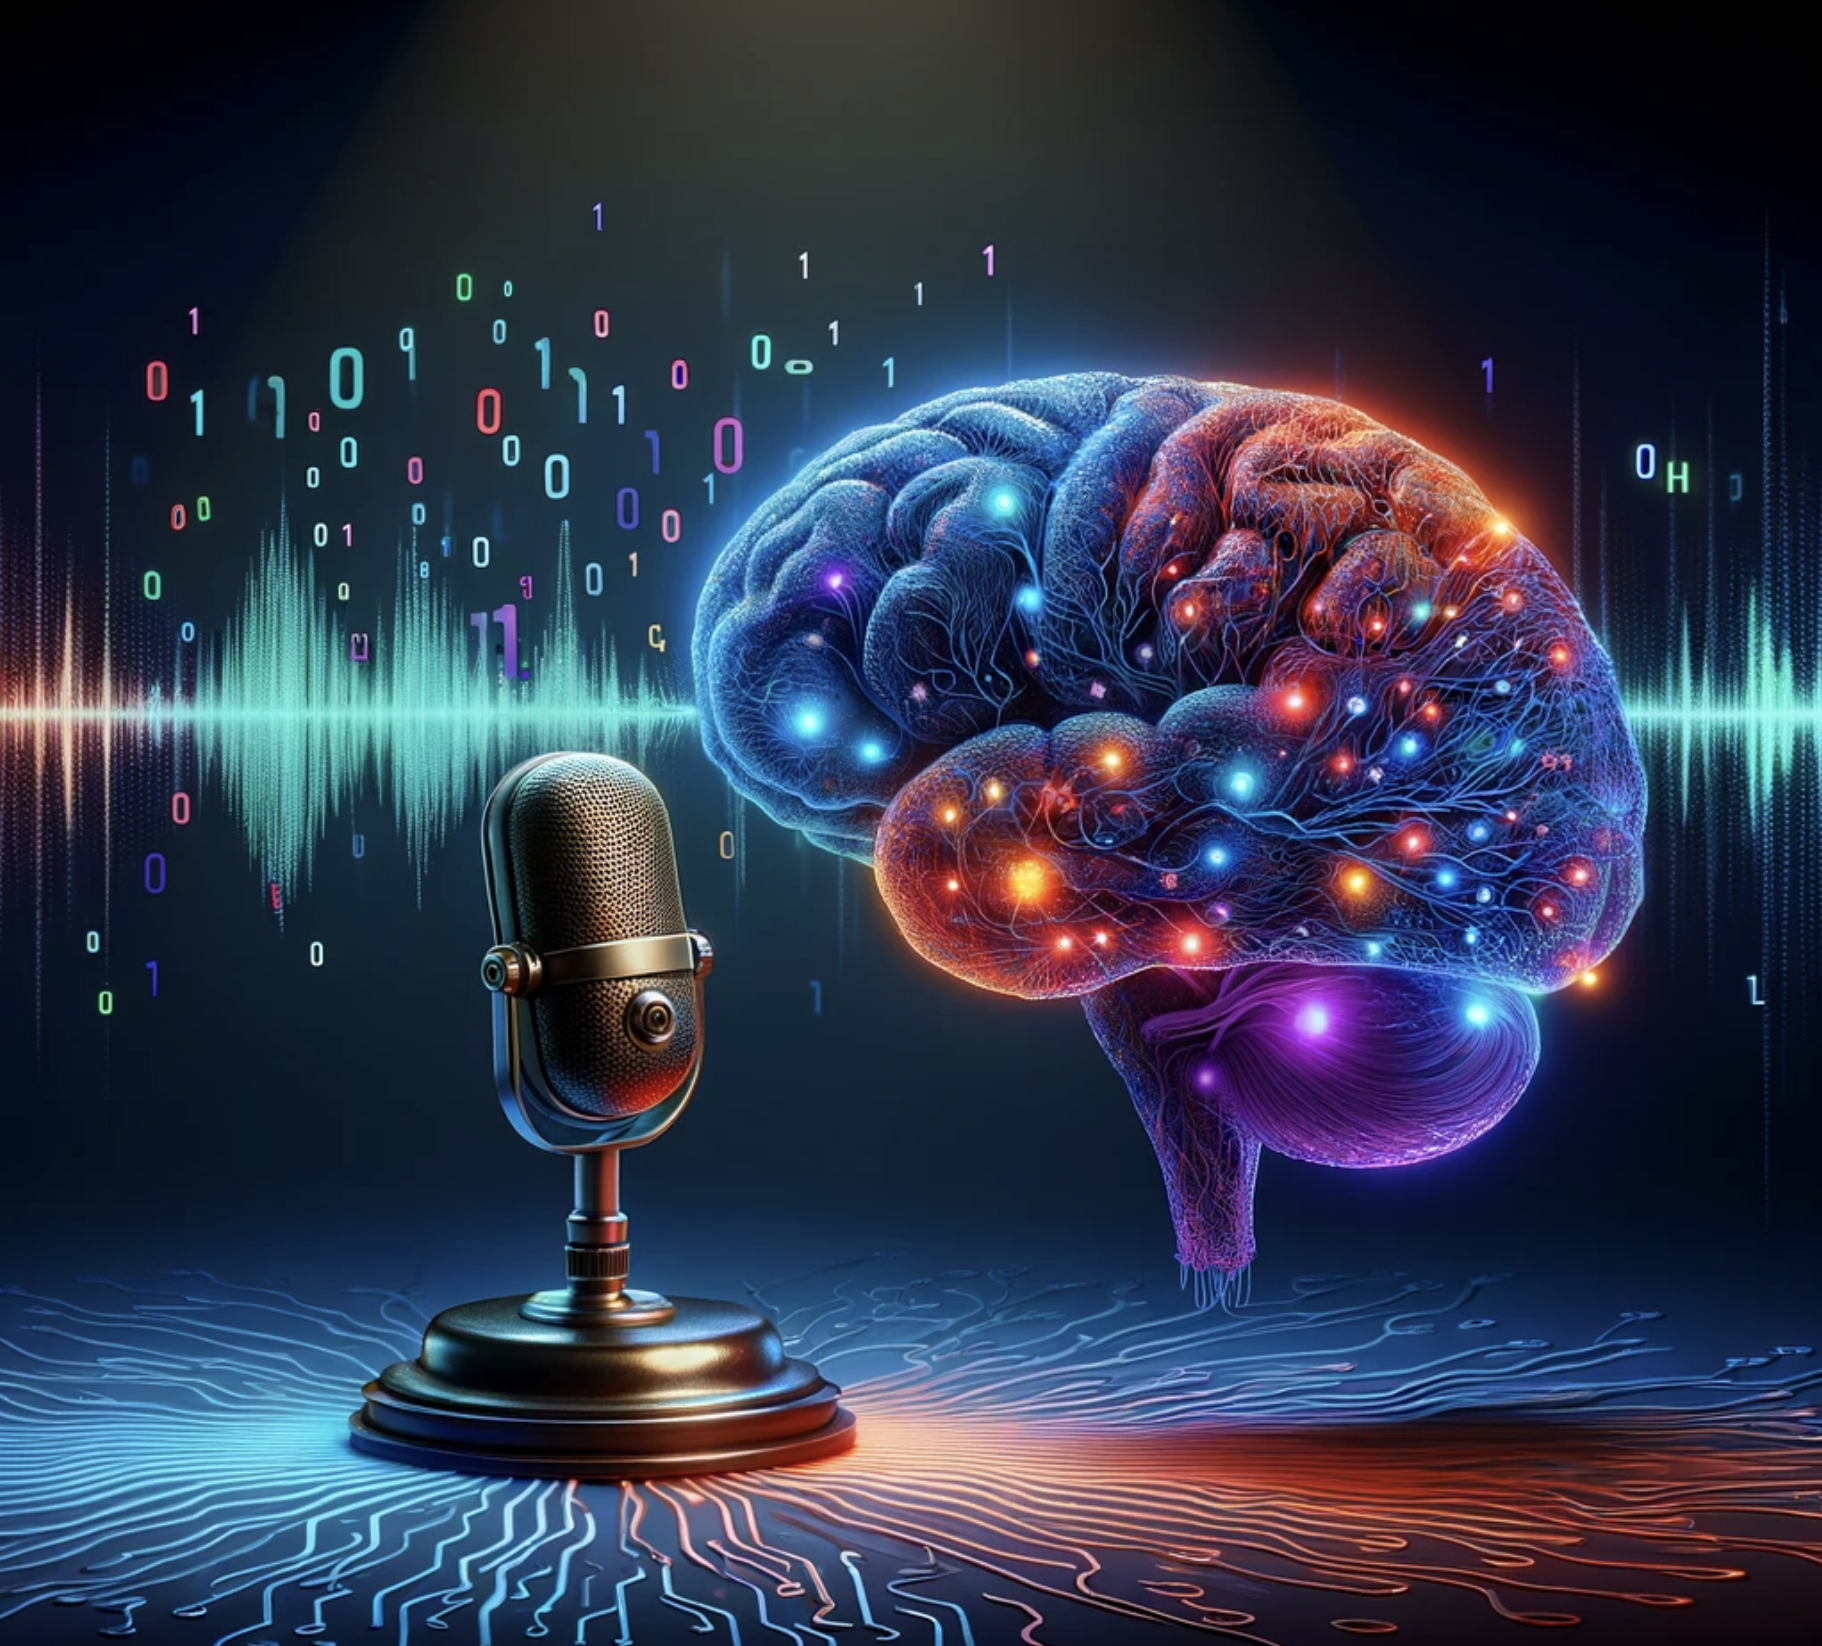
\includegraphics{_images/brain_podcast.png}

}

\caption{The image a podcaster's brain podcasting about brains}

\end{figure}%

We will encourage you to ask questions to the creators and to give them
\textbf{constructive} feedback. You will also be on the other end of
this feedback so, again, great opportunity to learn and to improve.
After listening to each podcast you all will vote the podcast on
different aspects (e.g., content, format) so that we can give the final
prizes based on the opinions of your peers.

Fonally, we will gather feedback from all students on the entire podcast
project so that we can improve it for the following year.

Let's make this session lively and engaging. Your participation and
feedback are crucial for the success of this activity!

\phantomsection\label{refs}
\begin{CSLReferences}{1}{0}
\bibitem[\citeproctext]{ref-amodio2014neuroscience}
Amodio, David M. 2014. {``The Neuroscience of Prejudice and
Stereotyping.''} \emph{Nature Reviews Neuroscience} 15 (10): 670--82.

\bibitem[\citeproctext]{ref-farah2017neuroscience}
Farah, Martha J. 2017. {``The Neuroscience of Socioeconomic Status:
Correlates, Causes, and Consequences.''} \emph{Neuron} 96 (1): 56--71.

\bibitem[\citeproctext]{ref-merabet2010neural}
Merabet, Lotfi B, and Alvaro Pascual-Leone. 2010. {``Neural
Reorganization Following Sensory Loss: The Opportunity of Change.''}
\emph{Nature Reviews Neuroscience} 11 (1): 44--52.

\bibitem[\citeproctext]{ref-meynell2013delusions}
Meynell, Letitia. 2013. {``Delusions of Gender: How Our Minds, Society,
and Neurosexism Create Difference. By Cordelia Fine. New York: WW Norton
\& Company, 2010.-Brain Storm: The Flaws in the Science of Sex
Differences. By Rebecca m. Jordan-Young Cambridge, Mass.: Harvard
University Press, 2010.''} \emph{Hypatia} 28 (3): 684--89.

\bibitem[\citeproctext]{ref-sohn2019decoding}
Sohn, Emily. 2019. {``Decoding Consciousness.''} \emph{Nature} 571
(7766): S2--5.

\bibitem[\citeproctext]{ref-yavari2018basic}
Yavari, Fatemeh, Asif Jamil, Mohsen Mosayebi Samani, Liliane Pinto
Vidor, and Michael A Nitsche. 2018. {``Basic and Functional Effects of
Transcranial Electrical Stimulation (tES)---an Introduction.''}
\emph{Neuroscience \& Biobehavioral Reviews} 85: 81--92.

\end{CSLReferences}




\end{document}
